%	1.4. Presentacion en Pantalla Electronica.
%	version 2018


\begin{frame}
  \begin{columns}
    \begin{column}{0.5\textwidth}
      \begin{block}{Un poco de historia...}
{\normalsize
        \begin{description}
        \item[1970] NASA investigaci\'on en como mostrar instrumentos
          de vuelo
        \item[1982]Boeing 767 con pantallas electr\'onicas de datos tipo \ac{CRT}
        \item[1990]Fines de la d\'ecada, pantallas \ac{LCD} reemplazan
          pantallas \ac{CRT}
        \item[Actualidad] La mayor\'ia de las aeronaves equipadas con
          pantallas \ac{LCD}
        \item[Futuro] Uso de pantallas tipo \ac{OLED}
        \end{description}
}
      \end{block}
    \end{column}

    \begin{column}{0.5\textwidth}
  \includegraphics[width=0.9\linewidth]{imagenes/1.4.pantalla.electronica/CRT.gif}

\vspace{3mm}

  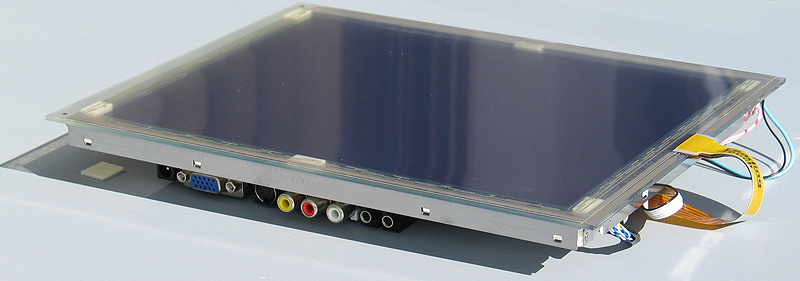
\includegraphics[width=0.8\linewidth]{imagenes/1.4.pantalla.electronica/LCD.jpg}

\vspace{3mm}

  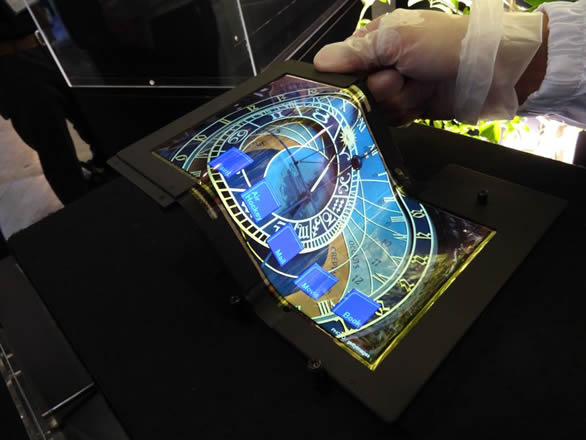
\includegraphics[width=0.7\linewidth]{imagenes/1.4.pantalla.electronica/foldable-oled-display.jpg}
    \end{column}
  \end{columns}

\end{frame}

\begin{frame}

  \begin{block}{ EIS (Electronic Instrument
      System)}

Ejemplos:

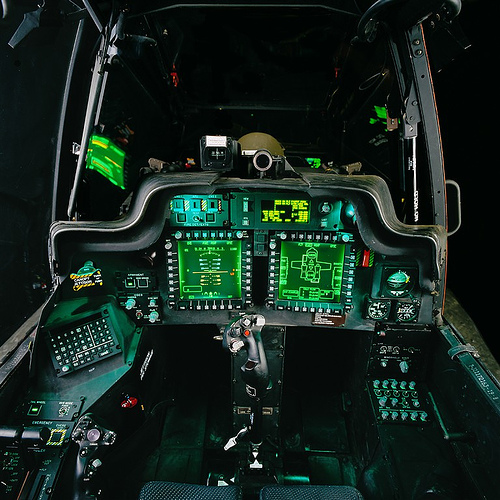
\includegraphics[width=0.34\textwidth]{imagenes/1.4.pantalla.electronica/apache.jpg}
\hspace{3mm}
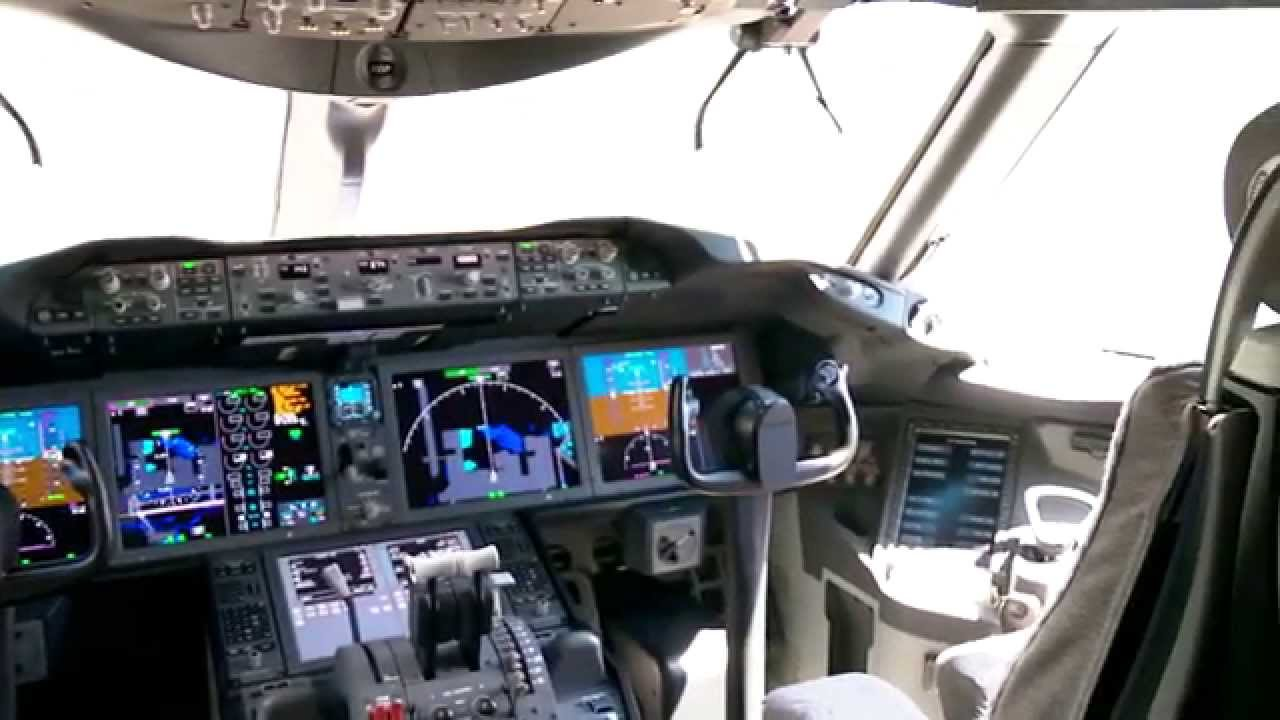
\includegraphics[width=0.55\textwidth]{imagenes/1.4.pantalla.electronica/dreamliner.jpg}

Helic\'optero Apache \hspace{25mm} Boeing 787 Dreamliner
  \end{block}

\end{frame}

\begin{frame}
  Una instalaci\'on EIS sigue la secuencia siguiente:

\vspace{3mm}


 Pantallas \qquad $\Longrightarrow$ \qquad
 Controles  \qquad $\Longrightarrow$ \qquad
 Procesadores de datos 

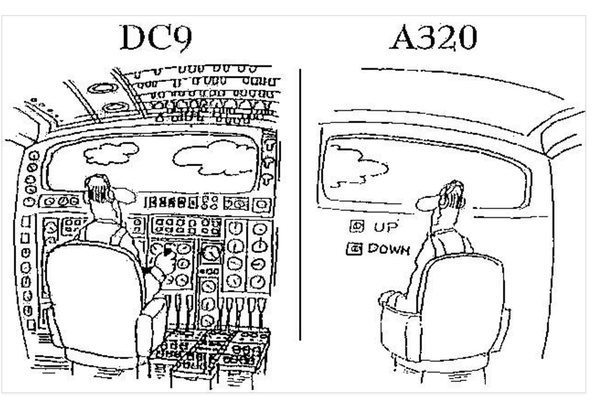
\includegraphics[width=0.85\textwidth]{imagenes/1.4.pantalla.electronica/efis_humor.png}

\end{frame}

\begin{frame}

  \begin{block}{Bus de datos}
{\small
    Las se\~nales que se env\'ian entre los distintos componentes del
    EIS se transmiten por una l\'inea de transmisi\'on digital
    denominada ``{\it Bus de Datos}". Las se\~nales transmitidas son
    peque\~nos pulsos de tensi\'on en c\'odigo binario (unos y
    ceros). Seg\'un el protocolo los unos y ceros se diferencian por
    tener valores distintos de tensiones positivas o negativas,
    variaciones de tensiones ascendentes o descendentes, falta de
    tensi\'on, etc. Los pusos de tensi\'on tienen duraciones
    extremadamente breves a fin de enviar una gran cantidad de
    informaci\'on en poco tiempo.
}
  \end{block}


  \begin{columns}
    \begin{column}{0.5\textwidth}
      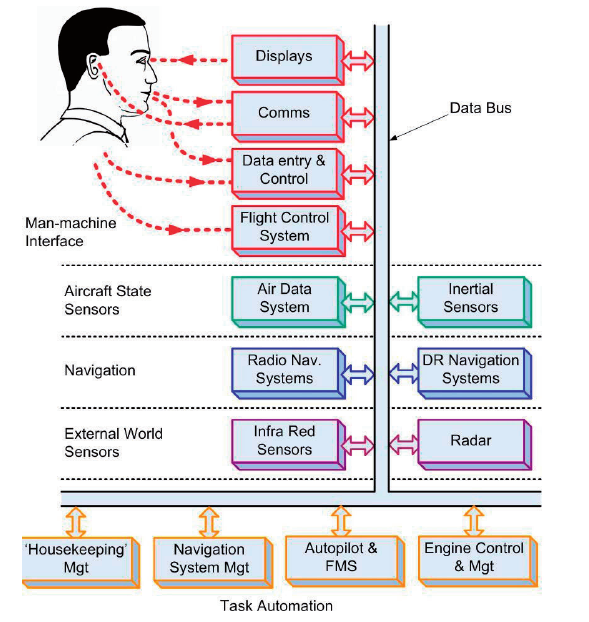
\includegraphics[width=\linewidth]{imagenes/1.2.clasificacion.instrumentos/tipos_instrumentos.png}

      {\tiny Referencia: \cite{Introduction_to_Avionics_Systems}}
    \end{column}
  \begin{column}{0.5\textwidth}
    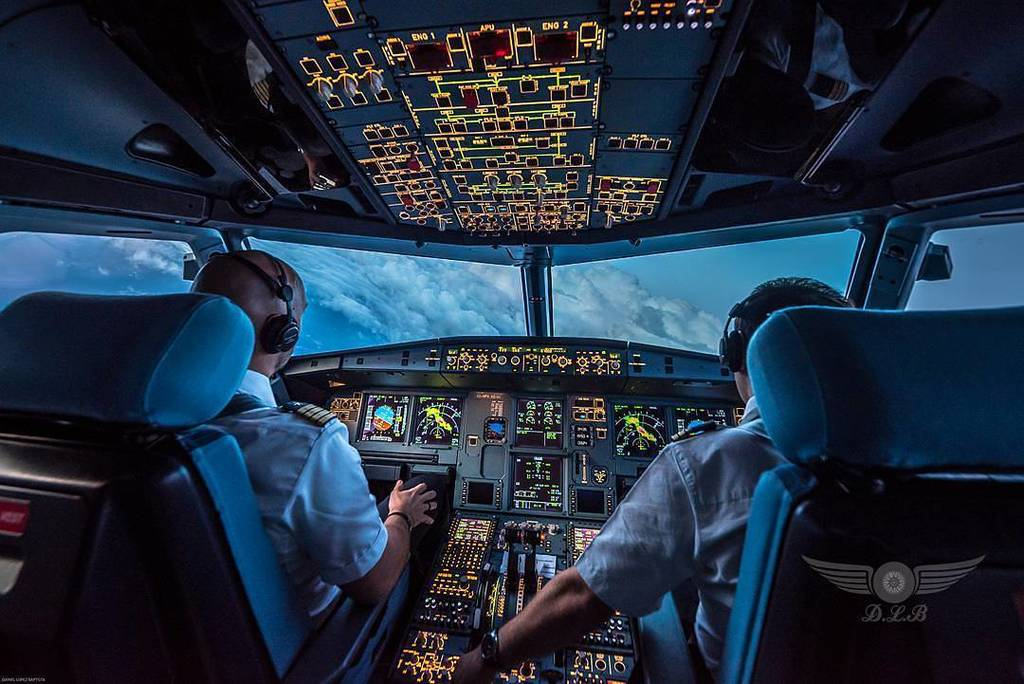
\includegraphics[width=\linewidth]{imagenes/1.2.clasificacion.instrumentos/glass_cockpit.jpg}
%    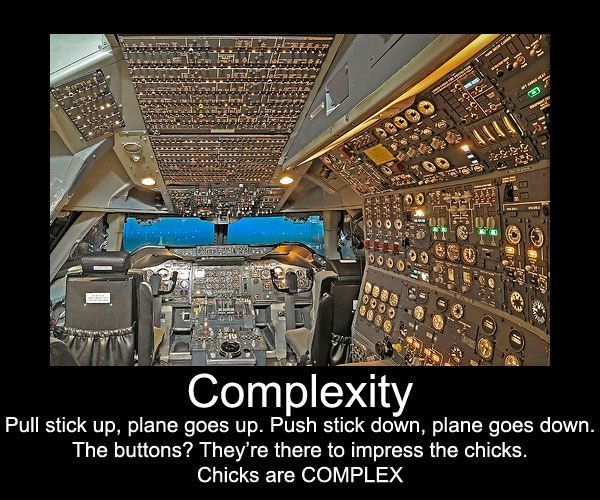
\includegraphics[width=\linewidth]{imagenes/1.2.clasificacion.instrumentos/humor_complejidad.jpg}
  \end{column}
  \end{columns}

\end{frame}

\begin{frame}

% Mientras que en el sistema de numeración decimal se usan diez dígitos (diez símbolos), en el binario se usan solo dos dígitos, el 0 y el 1. Un bit o dígito binario puede representar uno de esos dos valores: 0 o 1. 

% El bit es la unidad mínima de información empleada en informática, en cualquier dispositivo digital, o en la teoría de la información.

  \begin{exampleblock}{Buses de datos}
    \begin{itemize}
    \item Un sistema digital t\'ipico puede enviar se\~nales de pulsos
      con duraciones de 10 $\mu$seg

    \item Un sistema de bus digital usual en avi\'onica es el
      ARINC (Aeronautical Radio INCorporated), bajo cuya denominaci\'on existen una gran cantidad
      de protocolos de comunicaciones con diferencias b\'asicas en los
      par\'ametros de transmisi\'on y recepci\'on.

    \item ARINC es una gran empresa que desarrolla y opera
      sistemas y servicios para garantizar la eficiencia, el
      funcionamiento y el rendimiento de la aviaci\'on y la industria
      del transporte. Fue fundada en 1929 por cuatro grandes
      aerol\'ineas para proporcionar un \'unico licenciatario de
      comunicaciones fuera del gobierno.

    \item Por ejemplo, el ARINC 429 es una especificaci\'on que define
      como los equipos y sistemas de avi\'onica deber\'ian comunicarse
      entre s\'i. Emplea una transmisi\'on unidireccional conocida
      como Mark 33 DITS, de palabras de 32 bits a trav\'es de un
      par trenzado usando el formato bipolar RZ. Los mensajes se
      transmiten a una tasa de 12,5 o 100 kilobits por segundo. La
      transmisi\'on y la recepci\'on se realizan en puertos separados,
      por lo que es posible que se necesiten muchos cables en las
      aeronaves que utilizan una gran cantidad de sistemas de
      avi\'onica.
    \end{itemize}
  \end{exampleblock}

\end{frame}

\begin{frame}

  \begin{block}{Pantallas presentaci\'on de datos}

    \begin{itemize}
      \begin{multicols}{3}
      \item \ac{CRT}
      \item \ac{LCD}
      \item \ac{OLED}
      \end{multicols}
    \end{itemize}

	La imagen se forma por la uni\'on de muchos puntos (p\'ixeles). El p\'ixel es la menor 
unidad homog\'enea en color que forma parte de una imagen digital. 

      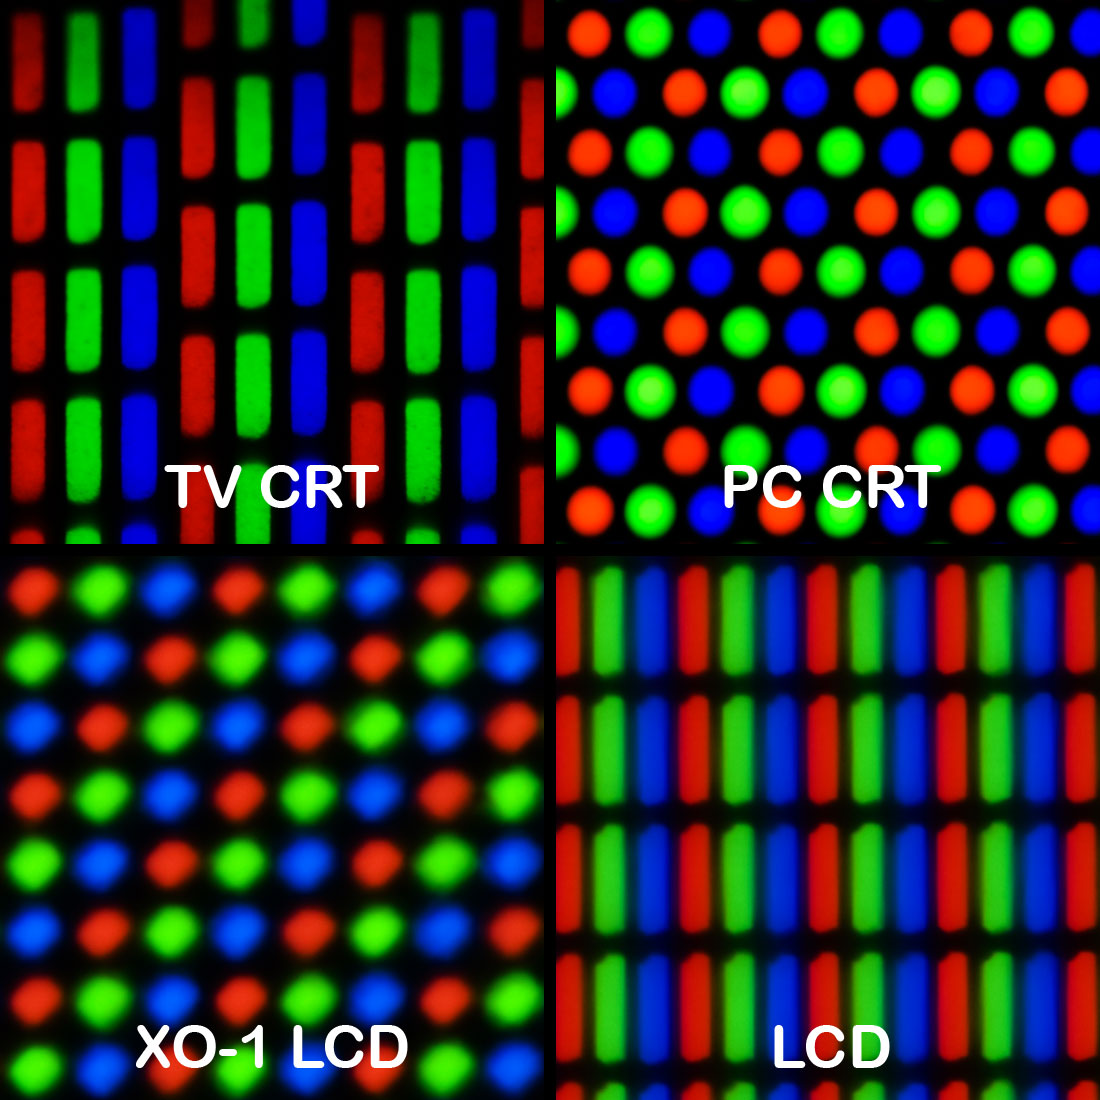
\includegraphics[width=0.4\linewidth]{imagenes/1.4.pantalla.electronica/Pixel_geometry_01_Pengo.jpg}


  \end{block}
  
\end{frame}

\begin{frame}

  \begin{block}{Pantalla \ac{CRT}}
    \begin{columns}[T]

      \begin{column}[T]{0.6\textwidth}
        \includegraphics[width=\linewidth]{imagenes/1.4.pantalla.electronica/CRT.gif}
      \end{column}

      \begin{column}[T]{0.4\textwidth}
	
        \begin{itemize}
{\footnotesize
        \item Los datos son enviados desde la computadora por medio
          del puerto de video hacia los circuitos del monitor.

        \item           Los circuitos internos los reciben y de acuerdo a lo
          especificado por la computadora controla los ca\~nones de
          electrones.

        \item           Estos ca\~nones lanzan haces electrones hacia la pantalla, la
          cu\'al tiene zonas sensibles fosforescentes (p\'ixeles) y al
          recibirlos emiten un peque\~no pulso de luz.

}
        \end{itemize}


      \end{column}
    \end{columns}

    \begin{itemize}
 {\footnotesize 
        \item           Para pantallas monocrom\'aticas integra solo un ca\~n\'on, para el
          monitor a color integra tres ca\~nones y cada uno controla un
          color (rojo, verde y azul), sistema RGB, los cuales
          mezclados determinan el color del p\'ixel en pantalla.

        \item           La trayectoria de los electrones en sentido vertical y
          horizontal hacia los p\'ixeles de la pantalla, es controlada
          por medio bobinas que emiten de campos magn\'eticos.

        \item           Como el tiempo que permanece encendido el p\'ixel es muy
          corto, el proceso se repite varias veces por segundo en toda
          la pantalla de manera horizontal y hacia abajo (entre 56 y
          120 veces); a este proceso se le denomina frecuencia y se
          mide en Hz o ciclos sobre segundo.

        \item           Lo anterior se repite aunque para el usuario la pantalla
          parezca est\'atica, \'esta se esta refrescando varias veces por
          segundo.
}
    \end{itemize}

  \end{block}
\end{frame}


\begin{frame}

  \begin{block}{Pantalla \ac{LCD}}
    \begin{columns}[T]

      \begin{column}[T]{0.5\textwidth}
        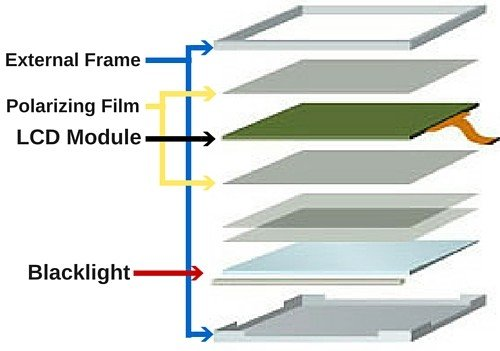
\includegraphics[width=\linewidth]{imagenes/1.4.pantalla.electronica/lcd_partes.jpg}
      \end{column}

      \begin{column}[T]{0.5\textwidth}
	
        \begin{itemize}
{\footnotesize
        \item Este dispositivo cuenta con un microprocesador encargado de determinar la posici\'on de cada píxel.

        \item Una pantalla LCD cuenta con 2 placas de vidrio, una de ellas esta iluminada de la parte trasera por una luz intensa procedente de l\'amparas CCFL (Cold-Cathode Fluorescent Lamps / L\'amparas fluorescentes de c\'atodo fr\'io), lo que permite el brillo en la pantalla.

        \item Una vez que se determina el p\'ixel a colorear, la celda cuenta con 3 sustancias propensas a recibir corriente y colorearse de alg\'un color básico (verde, rojo y azul) por medio de polarizaci\'on.

        \item La corriente que le llega a cada p\'ixel determina la saturaci\'on para cada color y as\'i se genera la gama de colores.

        \item El proceso se repite cada vez que cambian las im\'agenes en la pantalla.
	}
        \end{itemize}


      \end{column}
    \end{columns}

    \begin{itemize}
 {\footnotesize 
        \item           
	}
    \end{itemize}

  \end{block}
\end{frame}


\begin{frame}

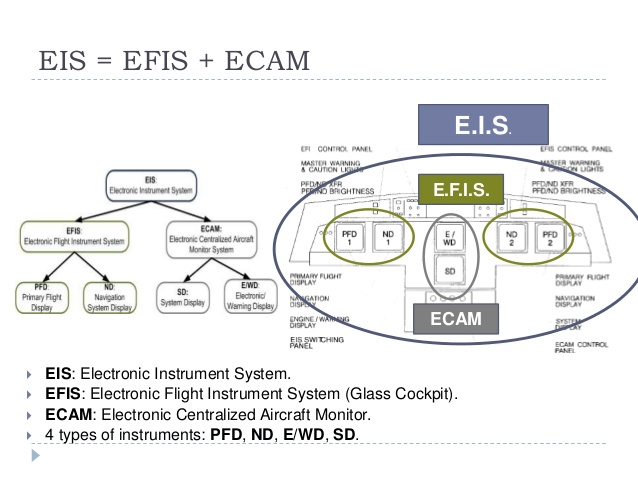
\includegraphics[width=0.85\textwidth]{imagenes/1.4.pantalla.electronica/efis.jpg}

\end{frame}

% \begin{frame}
  
%   \begin{bclogo}[couleur=blue!10, arrondi = 0.1,
% 	logo = \bccrayon, ombre = true
% 	]{Bclogo parece versatil}

% 	Box de prueba con bclogo
    
%   \end{bclogo}


% \end{frame}



\begin{frame}

     \begin{block}{ PFD: Primary Flight Display}
{\footnotesize
	% Presenta los siguientes instrumentos
	
	%  Airspeed Indicator, 
	%  Altimeter, 
	%  HSI (Horizontal Situation Indicator),
	%  VSI (Vertical Speed Indicator)
	

	El PFD reemplaza a los seis (6) instrumentos tradicionales

	Muestra la informaci\'on cr\'itica de vuelo 
	incluyendo velocidad, altitud,direcci\'on (heading)
	actitud y velocidad vertical

	Est\'a dise\~nado para mejorar las alertas al piloto
	al integrar informaci\'on en una sola pantalla

	Reduce el tiempo para monitorear otros instrumentos

	Alerta a los pilotos de condiciones potencialmente peligrosas
        cambiando el color o la forma en el display o mediante alertas
        de sonido. (baja velocidad, alta tasa de descenso) 
}
    \end{block}

 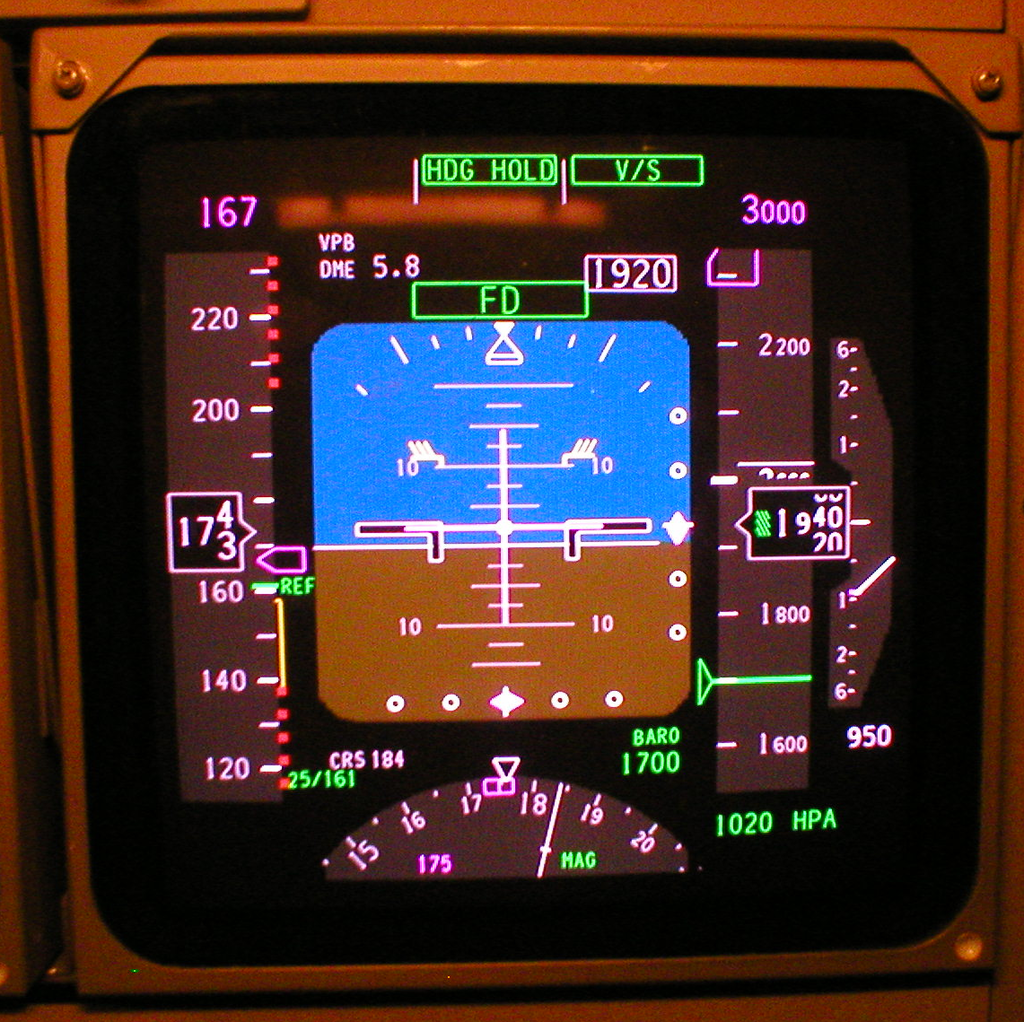
\includegraphics[width=3cm]{imagenes/1.4.pantalla.electronica/Primary_Flight_Display,_Boeing_747-400.png}\\
 

    \end{frame}      
    
\begin{frame}

  \begin{block}{ MDF: MultiFunction Display o ND (Navigation Display)}

    Informaci\'on para navegaci\'on (VOR, DME, ILS)

    Informaci\'on clim\'atica de m\'ultiples sistemas (radar a bordo,
    sensores de detecci\'on de rel\'ampagos)

    Idem al PFD el MDF puede cambiar color, forma y dar alertas
    sonoras

    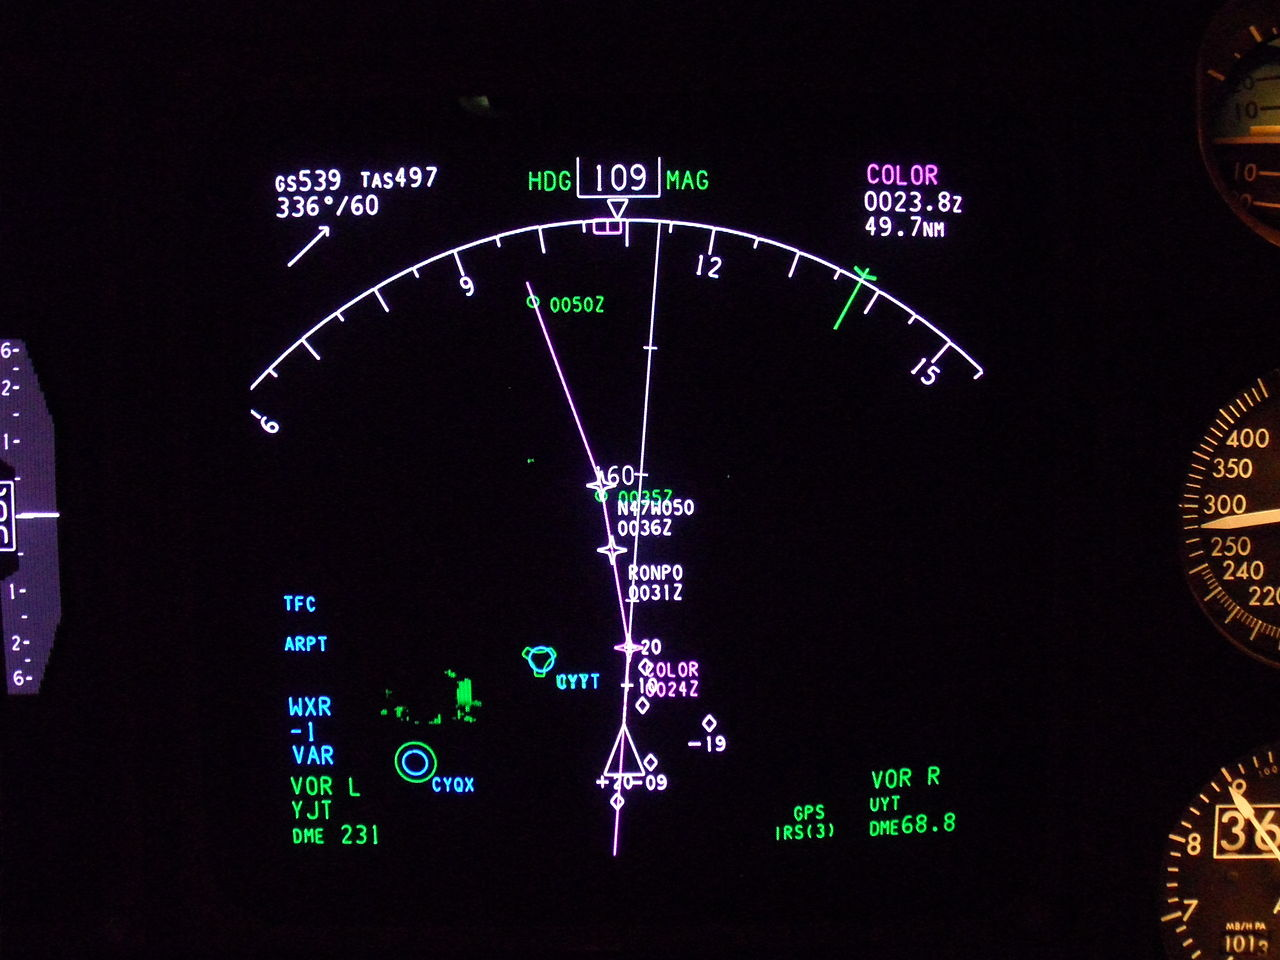
\includegraphics[width=6cm]{imagenes/1.4.pantalla.electronica/Navigation_Display_(ND)_on_Boeing_747-400.jpg}
  \end{block}
    \end{frame}      
    
\begin{frame}

  \begin{block}{ ECAM : Electronic Centralized Aircraft Monitor
    (Airbus) \\
     EICAS : Electronic Centralized Aircraft Monitor (Boeing)}


    Monitorear los sistemas de la aeronave: p.e. combustible, sistemas
    el\'ectricos y del motor

    Usualmente dos (2) pantallas, una arriba de la otra

    La pantalla superior muestra sistemas motores, posici\'on flaps
    cantidad de combustible e informaci\'on de alerta

    La pantalla inferior muestra diversos par\'ametros de sistemas

    Brinda alarmas en caso de malfuncionamiento

    P.e. en caso de p\'erdida de presi\'on de aceite en un motor, el
    ECAM hace sonar una alerta, cambia la pantalla a una que muestra
    el sistema de aceite y se\~nala la baja presi\'on con una caja
    roja.

  \end{block}
    \end{frame}

\begin{frame}
  \begin{tabular}{ccc}
	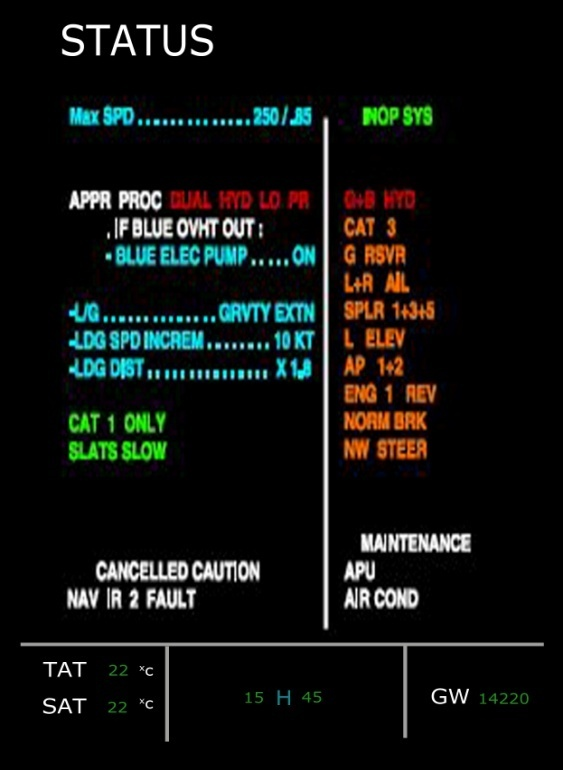
\includegraphics[width=4.5cm]{imagenes/1.4.pantalla.electronica/eicas_status.jpg}
	& \hspace{3mm} &
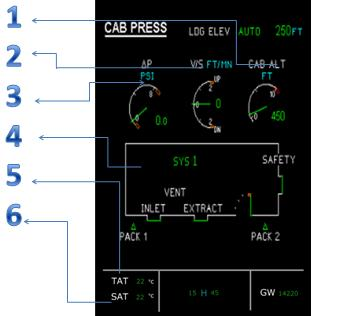
\includegraphics[width=6cm]{imagenes/1.4.pantalla.electronica/eicas_presion_cabina.jpg}
	\\
   	EICAS status & 
	& EICAS presi\'on cabina.  
% \parbox{\linewidth}{\tiny 1. Cabin altitude (height),
% 2. Vertical Speed (height/min),
% 3. Pressure,
% 4. Cabin,
% 5. True air temperature}
	\\
\end{tabular}

\end{frame}


\begin{frame}
  \begin{center}
    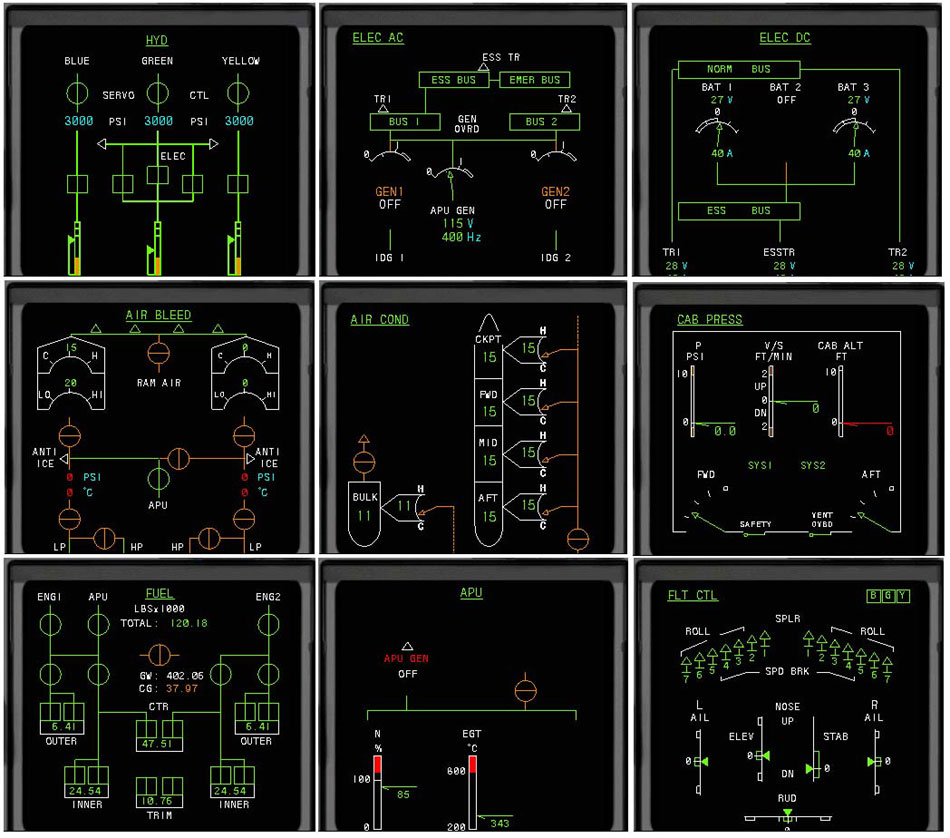
\includegraphics[width=0.65\textwidth]{imagenes/1.4.pantalla.electronica/ecam_airbus.jpg}

    \vspace{3mm}

    ECAM presentaci\'on
  \end{center}
\end{frame}

\begin{frame}

  \begin{block} { \ac{FMS}
%: Flight Management System
}

    Instrumentos para mantener el plan de vuelo (flight plan) permite
    a los pilotos modificarlo en vuelo

    Dada la posici\'on y el plan de vuelo, el  \ac{FMS} se encarga de guiar
    el avi\'on a lo largo del mismo, gestiona los diversos factores
    que afectan al vuelo del avi\'on, tanto la ruta que tiene que
    seguir, como los niveles \'optimos a los cuales volar para reducir
    el consumo y hacer un vuelo m\'as eficiente.


    Usualmente se presenta como una pantalla peque\~na y un teclado

    El \ac{FMS} se compone principalmente del \ac{CDU} y 
    el \ac{FMC}
  \end{block}


% {\bf Autopiloto (AP)}

% 	Computadora que permite que una aeronave se vuele a s\'i misma.

% 	Se utiliza habitualmente en vuelos de larga duraci\'on

% 	El piloto se encuentra presente siempre para monitorear
% 	y chequear que el vuelo se desarrolle seg\'un el plan


% \end{itemize}

\end{frame}

\begin{frame}


El piloto introduce los datos al \ac{FMC} a trav\'es de la \ac{CDU} que no es m\'as que un teclado 
y una pantalla que sirve para la comunicaci\'on entre el piloto y el \ac{FMC}. 
A trav\'es de la \ac{CDU} el piloto programa la ruta del vuelo, las \ac{SID}  
y las \ac{STAR}, as\'i como los puntos en las rutas donde el avi\'on debe ascender 
a niveles \'optimos seg\'un disminuye el peso del avi\'on.

    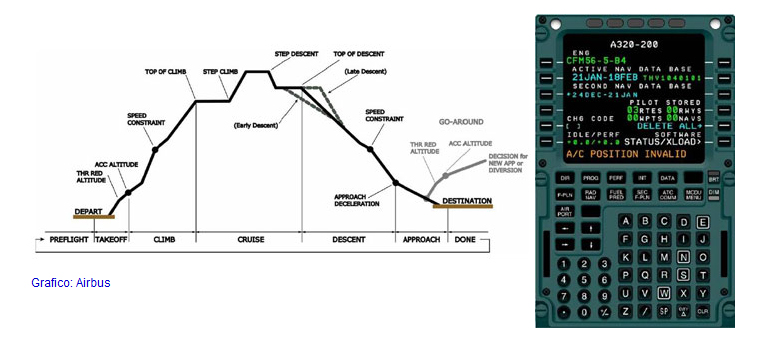
\includegraphics[width=0.9\textwidth]{imagenes/1.4.pantalla.electronica/fms_plan_vuelo.jpg}
  \end{frame}
  

\begin{frame}{Presentaci\'on en Pantalla Electr\'onica}
{\small
El \ac{FMC} adem\'as adquiere datos de muchos de los sistemas del avi\'on. Para empezar recibe informaci\'on de los inerciales, y de los \ac{GPS} para triangular la posici\'on del avi\'on y tener una posici\'on a\'un m\'as exacta de donde se encuentra el avi\'on.

El \ac{FMS} tiene principalmente dos bases de datos. Una base de datos de navegaci\'on, donde est\'an almacenadas las rutas, aerov\'ias, \ac{SID}, \ac{STARS}, as\'i como las frecuencias de las radio ayudas a la navegaci\'on que va a sintonizar autom\'aticamente a lo largo de la ruta. Esta base de datos se renueva cada 28 d\'ias para poder estar actualizada cuando se producen cambios en los espacios a\'ereos o se modifican procedimientos de aproximaci\'on. 
El \ac{FMC} es capaz de guardar dos (2)  bases de datos de navegaci\'on.

La otra base de datos es de performance del avi\'on. Esta base de datos contiene informaci\'on de los niveles \'optimos de vuelo dependiendo del peso del avi\'on. Los consumos que tiene el avi\'on para cada peso y nivel de vuelo. Las predicciones de ascenso y descenso del avi\'on.

Como el avi\'on va envejeciendo a lo largo de su vida y disminuyendo sus performance, el \ac{FMS} admite un valor de degradaci\'on de las performance que se introduce en la p\'agina principal del \ac{CDU} para que de unas previsiones de combustibles m\'as reales seg\'un el avi\'on se va haciendo ``mayor''
}
\end{frame}


\begin{frame}

{\small
Con el tiempo el \ac{FMS} ha ido mejorando y abarcando nuevas posibilidades. As\'i Airbus cambia el nombre 
al \ac{CDU} y le ha pasado a llamar \ac{MCDU}. Ahora no solamente se puede acceder 
al \ac{FMC} a trav\'es del teclado de la \ac{CDU} si no a una infinidad de nuevos servicios.

Mediante el \ac{MCDU} se accede al \ac{ATSU}, \ac{AIDS}, \ac{CFDS} y al \ac{FMS} 
comentado hasta ahora y llamado por Airbus \ac{FMGS}.

\begin{itemize}
\item El \ac{ATSU} es el acceso al Acars o sistema de comunicaciones
  tanto con la compa\~n\'ia como con el control a\'ereo. A trav\'es de
  esta opci\'on se recibe desde la hoja de carga, cualquier mensaje
  escrito que envie la compa\~n\'ia, hasta la autorizaci\'on para
  ingresar a otro pa\'is.

\item   El \ac{CFDS} es usado principalmente por el personal de
  mantenimiento.  En el est\'an los reportes de mantenimiento del
  vuelo, y las aver\'ias que haya tenido el avi\'on, por muy
  peque\~nas o temporales que hayan sido (aunque haya sido un fallo
  temporal de cualquier fusible por menos de 1 sg se queda
  registrado).

\item   El \ac{AIDS} es otra herramienta que maneja mantenimiento, sirve
  para interrogar y realizar TEST a cualquier sistema del avi\'on para
  conocer en qu\'e estado de operatividad se encuentra.
\end{itemize}


}
\end{frame}

\begin{frame}

    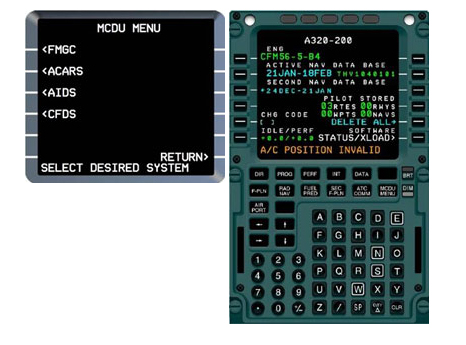
\includegraphics[width=0.9\textwidth]{imagenes/1.4.pantalla.electronica/mcdu.jpg}

\end{frame}

\begin{frame}
  
Las pantallas \ac{OLED} consisten en paneles muy delgados que permiten un ahorro
de peso y espacio, la potencia que necesitan es muy reducida y poseen posibilidades
de emplearse como pantallas flexibles aunque, tambi\'en poseen limitaciones.
El principal problema es la madurez de la tecnolog\'ia que no es suficiente
para el uso en avi\'onica, su brillo no es suficiente y su vida \'util, reducida.




\url{http://www.optinvent.com/wp-content/uploads/2016/03/Odicis_IDW10final_2.pdf}

\end{frame}